\documentclass[12pt]{amsart}
\usepackage{amsfonts,amsmath,amsthm,amssymb}
\usepackage[dvipsnames]{xcolor}
\usepackage{tikz}
\usetikzlibrary{matrix}
\usepackage[colorlinks]{hyperref}

\begin{document}

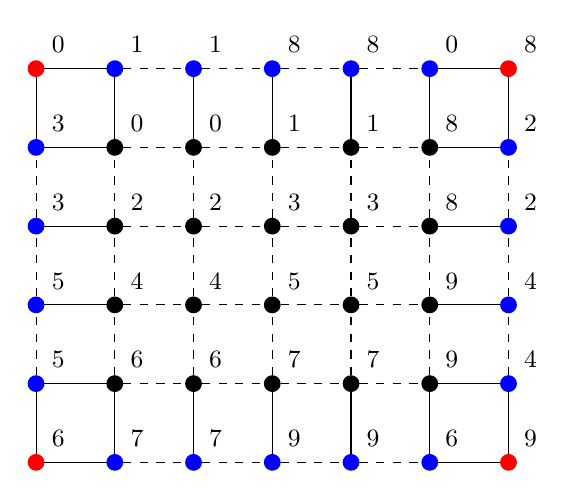
\begin{tikzpicture}[scale=1, every label/.append style={font=\small}]
\tikzstyle{pt}=[draw,shape=circle,inner sep=2pt,fill=black];
%1
\begin{scope}[]
	\node[pt,red] (1) at (0,0) [label=above right:6] {};
	\node[pt,blue] (2) at (0,1) [label=above right:5] {};
	\node[pt,blue] (3) at (0,2) [label=above right:5] {};
	\node[pt,blue] (4) at (0,3) [label=above right:3] {};
	\node[pt,blue] (5) at (0,4) [label=above right:3] {};
	\node[pt,red] (6) at (0,5) [label=above right:0] {};
	\draw (1) -- (2) (5) -- (6);
	\draw[dashed] (2) -- (3) -- (4) -- (5);
	\draw (1) -- +(1,0) (2) -- +(1,0) (3) -- +(1,0) (4) -- +(1,0) (5) -- +(1,0) (6) -- +(1,0);
\end{scope}
%2
\begin{scope}[shift={(1,0)}]
	\node[pt,blue] (1) at (0,0) [label=above right:7] {};
	\node[pt] (2) at (0,1) [label=above right:6] {};
	\node[pt] (3) at (0,2) [label=above right:4] {};
	\node[pt] (4) at (0,3) [label=above right:2] {};
	\node[pt] (5) at (0,4) [label=above right:0] {};
	\node[pt,blue] (6) at (0,5) [label=above right:1] {};
	\draw (1) -- (2) (5) -- (6);
	\draw[dashed] (2) -- (3) -- (4) -- (5);
	\draw[dashed] (1) -- +(1,0) (2) -- +(1,0) (3) -- +(1,0) (4) -- +(1,0) (5) -- +(1,0) (6) -- +(1,0);
\end{scope}
%3
\begin{scope}[shift={(2,0)}]
	\node[pt,blue] (1) at (0,0) [label=above right:7] {};
	\node[pt] (2) at (0,1) [label=above right:6] {};
	\node[pt] (3) at (0,2) [label=above right:4] {};
	\node[pt] (4) at (0,3) [label=above right:2] {};
	\node[pt] (5) at (0,4) [label=above right:0] {};
	\node[pt,blue] (6) at (0,5) [label=above right:1] {};
	\draw (1) -- (2) (5) -- (6);
	\draw[dashed] (2) -- (3) -- (4) -- (5);
	\draw[dashed] (1) -- +(1,0) (2) -- +(1,0) (3) -- +(1,0) (4) -- +(1,0) (5) -- +(1,0) (6) -- +(1,0);
\end{scope}
%4
\begin{scope}[shift={(3,0)}]
	\node[pt,blue] (1) at (0,0) [label=above right:9] {};
	\node[pt] (2) at (0,1) [label=above right:7] {};
	\node[pt] (3) at (0,2) [label=above right:5] {};
	\node[pt] (4) at (0,3) [label=above right:3] {};
	\node[pt] (5) at (0,4) [label=above right:1] {};
	\node[pt,blue] (6) at (0,5) [label=above right:8] {};
	\draw (1) -- (2) (5) -- (6);
	\draw[dashed] (2) -- (3) -- (4) -- (5);
	\draw[dashed] (1) -- +(1,0) (2) -- +(1,0) (3) -- +(1,0) (4) -- +(1,0) (5) -- +(1,0) (6) -- +(1,0);
\end{scope}
%5
\begin{scope}[shift={(4,0)}]
	\node[pt,blue] (1) at (0,0) [label=above right:9] {};
	\node[pt] (2) at (0,1) [label=above right:7] {};
	\node[pt] (3) at (0,2) [label=above right:5] {};
	\node[pt] (4) at (0,3) [label=above right:3] {};
	\node[pt] (5) at (0,4) [label=above right:1] {};
	\node[pt,blue] (6) at (0,5) [label=above right:8] {};
	\draw (1) -- (2) (5) -- (6);
	\draw[dashed] (2) -- (3) -- (4) -- (5);
	\draw[dashed] (1) -- +(1,0) (2) -- +(1,0) (3) -- +(1,0) (4) -- +(1,0) (5) -- +(1,0) (6) -- +(1,0);
\end{scope}
%6
\begin{scope}[shift={(5,0)}]
	\node[pt,blue] (1) at (0,0) [label=above right:6] {};
	\node[pt] (2) at (0,1) [label=above right:9] {};
	\node[pt] (3) at (0,2) [label=above right:9] {};
	\node[pt] (4) at (0,3) [label=above right:8] {};
	\node[pt] (5) at (0,4) [label=above right:8] {};
	\node[pt,blue] (6) at (0,5) [label=above right:0] {};
	\draw (1) -- (2) (5) -- (6);
	\draw[dashed] (2) -- (3) -- (4) -- (5);
	\draw (1) -- +(1,0) (2) -- +(1,0) (3) -- +(1,0) (4) -- +(1,0) (5) -- +(1,0) (6) -- +(1,0);
\end{scope}
%7
\begin{scope}[shift={(6,0)}]
	\node[pt,red] (1) at (0,0) [label=above right:9] {};
	\node[pt,blue] (2) at (0,1) [label=above right:4] {};
	\node[pt,blue] (3) at (0,2) [label=above right:4] {};
	\node[pt,blue] (4) at (0,3) [label=above right:2] {};
	\node[pt,blue] (5) at (0,4) [label=above right:2] {};
	\node[pt,red] (6) at (0,5) [label=above right:8] {};
	\draw (1) -- (2) (5) -- (6);
	\draw[dashed] (2) -- (3) -- (4) -- (5);
\end{scope}
\end{tikzpicture}

\end{document}